\documentclass{sig-alternate}

\usepackage[utf8]{inputenc}
\usepackage[activate=compatibility]{microtype}

% autoref command
\usepackage[hyphens]{url}
\usepackage[pdftex,urlcolor=black,colorlinks=true,linkcolor=black,citecolor=black]{hyperref}
\def\sectionautorefname{Section}
\def\subsectionautorefname{Subsection}

% Graphics
\usepackage{graphicx}
\usepackage{subfig}
\usepackage[font=small]{caption}
\captionsetup[figure]{name=Figure}
\usepackage{subcaption}

\usepackage{amsmath}
\usepackage{enumitem}
\usepackage{pbox}
\usepackage{color}
\definecolor{light-gray}{gray}{0.8}

% todo macro
\usepackage{color}
\newcommand{\todo}[1]{\noindent\textcolor{red}{{\bf \{TODO}: #1{\bf \}}}}

% nicer looking Google+
\usepackage{xspace}
\DeclareRobustCommand{\googleplus}{\mbox{Google\hspace{0em}\raisebox{.28ex}{\tiny\bf +}\kern-0.2ex}\xspace}

\DeclareRobustCommand{\plusone}{\mbox{\hspace{0em}\raisebox{.28ex}{\tiny\bf +}\kern-0.2ex 1}\xspace}

% listings and Verbatim environment
\usepackage{fancyvrb}
\usepackage{relsize}
\usepackage{listings}
\usepackage{verbatim}
\newcommand{\defaultlistingsize}{\fontsize{8pt}{9.5pt}}
\newcommand{\inlinelistingsize}{\fontsize{8pt}{11pt}}
\newcommand{\smalllistingsize}{\fontsize{7.5pt}{9.5pt}}
\newcommand{\listingsize}{\defaultlistingsize}
\RecustomVerbatimCommand{\Verb}{Verb}{fontsize=\inlinelistingsize}
\RecustomVerbatimEnvironment{Verbatim}{Verbatim}{fontsize=\defaultlistingsize}
\lstset{frame=lines,captionpos=b,numberbychapter=false,escapechar=§,
        aboveskip=2em,belowskip=1em,abovecaptionskip=0.5em,belowcaptionskip=0.5em,
        framexbottommargin=-1em,basicstyle=\ttfamily\listingsize\selectfont}

% use Courier from this point onward
\let\oldttdefault\ttdefault
\renewcommand{\ttdefault}{pcr}
\let\oldurl\url
\renewcommand{\url}[1]{\inlinelistingsize\oldurl{#1}}

\lstdefinelanguage{JavaScript}{
  keywords={push, typeof, new, true, false, catch, function, return, null, catch, switch, var, if, in, while, do, else, case, break},
  keywordstyle=\bfseries,
  ndkeywords={class, export, boolean, throw, implements, import, this},
  ndkeywordstyle=\color{darkgray}\bfseries,
  identifierstyle=\color{black},
  sensitive=false,
  comment=[l]{//},
  morecomment=[s]{/*}{*/},
  commentstyle=\color{darkgray},
  stringstyle=\color{red},
  morestring=[b]',
  morestring=[b]"
}

% linewrap symbol
\definecolor{grey}{RGB}{130,130,130}
\newcommand{\linewrap}{\raisebox{-.6ex}{\textcolor{grey}{$\hookleftarrow$}}}

\hyphenation{Wikistream Wikipedia Wikipedias}

%\def\baselinestretch{0.99}

\begin{document}

% --- Author Metadata here ---
\conferenceinfo{World Wide Web Conference}{'13 Rio de Janeiro, Brazil}
\CopyrightYear{2013} % Allows default copyright year (20XX) to be over-ridden - IF NEED BE.
%\crdata{0-12345-67-8/90/01}  % Allows default copyright data (0-89791-88-6/97/05) to be over-ridden - IF NEED BE.
% --- End of Author Metadata ---


\title{To Crop, Or Not to Crop: Creating Online Media Galleries}

\numberofauthors{2}\author{
\alignauthor
Thomas Steiner\\
	\affaddr{Google Germany GmbH}\\
	\affaddr{ABC-Str. 19}\\
	\affaddr{20354 Hamburg, Germany}\\
	\email{tomac@google.com} 
\alignauthor
Christopher Chedeau\\
	\affaddr{Facebook, Inc.}\\
	\affaddr{1601 Willow Road}\\
	\affaddr{Menlo Park, CA, 94025, USA}\\
	\email{vjeux@facebook.com} 
}
\maketitle

\begin{abstract}
We have developed an application for the automatic generation of
media galleries that visually and audibly summarize events
based on media items like videos and photos from multiple social networks.
We have evaluated different media gallery styles with online surveys 
and examined their pros and cons.
Besides the survey results, our contribution is also the application itself,
where media galleries of different styles can be created on-the-fly.
A~demo is available at
\url{http://social-media-illustrator.herokuapp.com/}.
\end{abstract}

\vspace{-1mm}
\category{H.3.3}{Information Search and Retrieval}{Clustering}

\vspace{-2mm}
\terms{Algorithms}

\vspace{-2mm}
\keywords{Media Galleries, Event Summarization, Social Networks}

\section{Introduction}

Media galleries (see \autoref{fig:media-gallery} for two examples)
help people consume larger, however not overwhelmingly huge,
amounts of media items in an ideally pleasing and aesthetic way.
These media items may, or, more commonly, may not be ordered,
besides an intrinsic chronologic order.
In the context of our work on summarizing events
based on microposts and media items stemming from
multiple social networks, we have created means
to first \emph{extract} event-related media items
from multiple social networks, second, to
\emph{deduplicate} near- and exact-duplicate media items,
third, to \emph{cluster} them by visual similarity, and
finally, to \emph{rank} the resulting media item clusters
according to well-defined ranking criteria.
In this paper, we treat the challenge of \emph{compiling}
ranked media item clusters in media galleries in ways
such that the ranking-implied order is respected.
Previously, we have defined~\cite{steiner2012definingaesthetic}
aesthetic principles for automatic media gallery layout,
which we now apply to different media gallery types.

\section{Media Gallery Styles}

Media galleries---in contrast to free-form digital media collages---%
necessarily display media items in a~grid-like manner.
The crucial question is thus, whether the media items' aspect ratios
should be respected, or whether they should be cropped to square,
or other aspect ratios (\emph{e.g.}, 4:3 or 16:9).
Respecting the aspect ratio has the obvious advantage that the media items
do not need to be potentially lossily cropped,
however, makes the creation of a~media gallery
that does not look ragged or frayed harder.

\subsection{Strict Order, Equal Size}

\subsection{Loose Order, Varying Size}

\section{Discussion}

\section{Evaluation}

Evaluating subjective data, like \emph{the} correct presentation form
for a~set of media items, is a~challenging task.
For different users, there may be different optimal settings.
A~common subjective evaluation technique
is the Mean~Opinion Score (MOS,~\cite{itu1998mos}).
Traditionally, MOS is used for conducting subjective evaluations
of telephony network transmission quality,
however, recently MOS has also found
wider usage in the multimedia community
for evaluating \emph{per se} subjective things
like perceived quality from a~user perspective. 
Therefore, a~set of standard subjective tests are conducted,
where a~number of users rate the quality of test samples
with scores ranging from 1 (worst) to 5 (best).
The actual MOS is then the arithmetic mean of all individual scores.

\section{Conclusions and Future Work}

\begin{figure*}[t!]
  \centering
  \subfloat[Strict order, equal size]{
    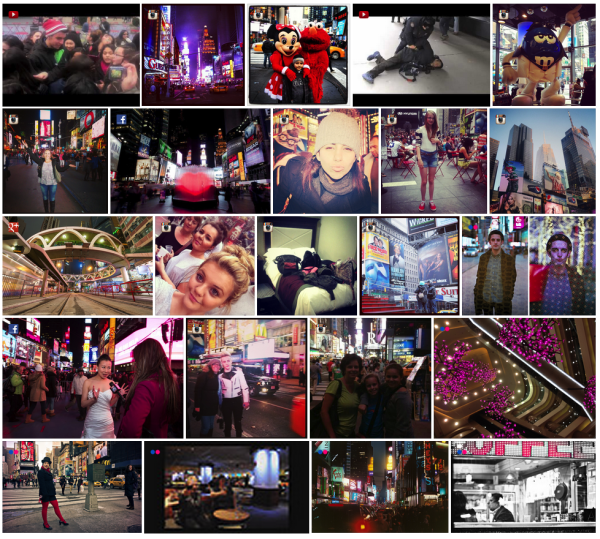
\includegraphics[height=5cm]{equal-size.png}
    \label{fig:a}
  }                
  \subfloat[Loose order, varying size (cropped)]{
    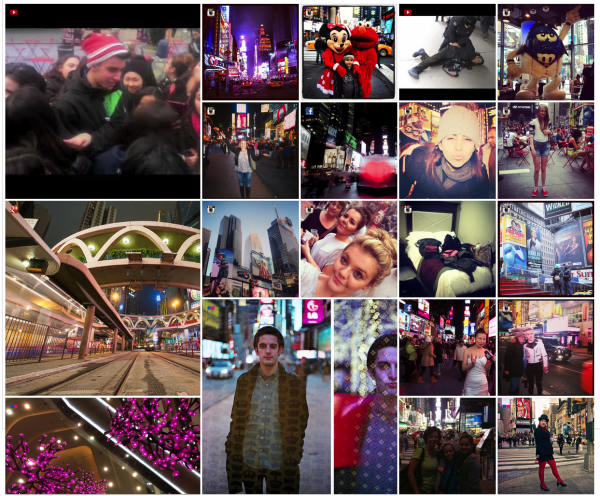
\includegraphics[height=5cm]{different-size.png}
    \label{fig:b}
  }
  \caption{Two different kinds of media galleries visualizing a~gathering at Times Square, New York on February 8, 2013}
  \label{fig:media-gallery}  
\end{figure*}



\bibliographystyle{abbrv}
\bibliography{www2013poster}

\end{document}